%-----------------------------------------------------------------------
% IR-SAM: Interpreter-Bounded, Sound Automated Repair of Injection
% Vulnerabilities in Java and Python.
%
% IEEE conference (IEEEtran).  Compile with:  tectonic main.tex
%-----------------------------------------------------------------------
\documentclass[conference]{IEEEtran}
\IEEEoverridecommandlockouts

\usepackage{cite}
\usepackage{amsmath,amssymb,amsfonts,amsthm}
\usepackage{algorithm}
\usepackage{algpseudocode}
\usepackage{graphicx}
\usepackage{textcomp}
\usepackage{xcolor}
\usepackage{listings}
\usepackage{booktabs}
\usepackage{multirow}
\usepackage{url}
\usepackage{hyperref}
\usepackage{tikz}
\usepackage{pgfplots}
\usepackage{enumitem}
\usepackage{balance}
\usetikzlibrary{positioning,arrows.meta,shapes.geometric,fit,backgrounds}
\pgfplotsset{compat=1.18}

\hypersetup{colorlinks=true,linkcolor=blue!60!black,citecolor=blue!60!black,
            urlcolor=blue!60!black}

%------- code listing styles ------------------------------------------
\definecolor{cBg}{rgb}{0.97,0.97,0.98}
\definecolor{cKw}{rgb}{0.05,0.05,0.55}
\definecolor{cStr}{rgb}{0.55,0.10,0.10}
\definecolor{cCom}{rgb}{0.30,0.45,0.30}

\lstdefinestyle{code}{
  basicstyle=\ttfamily\scriptsize,
  keywordstyle=\color{cKw}\bfseries,
  stringstyle=\color{cStr},
  commentstyle=\color{cCom}\itshape,
  backgroundcolor=\color{cBg},
  breaklines=true,
  columns=fullflexible,
  showstringspaces=false,
  frame=single,
  xleftmargin=2mm,
  numbers=none,
  language=Java
}
\lstdefinelanguage{Lean}{
  morekeywords={theorem,axiom,def,lemma,fun,let,in,match,with,by,
                exact,intro,rfl,structure,inductive,instance,
                example,namespace,end,if,then,else,where,
                Prop,Type,List,Bool},
  morecomment=[s]{/-}{-/},
  morecomment=[l]{--},
  morestring=[b]"
}
\lstdefinelanguage{YAML}{
  morekeywords={true,false,null,name,binder,host,sink,grammar,
                obligation,rewrite,gate,allowlist,parameters},
  sensitive=false,
  morecomment=[l]{\#},
  morestring=[b]'
}

%------- theorems ------------------------------------------------------
\newtheorem{definition}{Definition}
\newtheorem{theorem}{Theorem}
\newtheorem{lemma}{Lemma}
\newtheorem{corollary}{Corollary}
\newtheorem{proposition}{Proposition}

\def\BibTeX{{\rm B\kern-.05em{\sc i\kern-.025em b}\kern-.08em
    T\kern-.1667em\lower.7ex\hbox{E}\kern-.125emX}}

\newcommand{\IRSAM}{\textsc{IR-SAM}}
\newcommand{\sig}{\textsc{SIG}}
\newcommand{\sigP}{\ensuremath{G_{\!\sig}}}
\newcommand{\phisig}{\ensuremath{\varphi}}
\newcommand{\todo}[1]{\textcolor{red}{\textbf{[TODO: #1]}}}
\newcommand{\rqref}[1]{RQ\ref{rq:#1}}

\begin{document}

\title{IR-SAM: Interpreter-Bounded, Sound Automated Repair\\of Injection
Vulnerabilities in Java and Python\\with a Mechanised Soundness Argument}

\author{
  \IEEEauthorblockN{Anonymous Authors}
  \IEEEauthorblockA{Affiliation Withheld for Double-Blind Review\\
                    \texttt{ir-sam@anonymous.org}}
}

\maketitle

%======================================================================
\begin{abstract}
Automated remediation of injection vulnerabilities (CWE-89, CWE-78,
CWE-90, CWE-643, CWE-1336) has been dominated by neural sequence-to-
sequence patchers that hallucinate, by SAST autofix rules that
over-rewrite, and by LLM-driven repair loops that lack any soundness
criterion. We present \IRSAM, an \emph{interpreter-bounded} repair
engine for Java and Python that combines four ideas:
(i)~a Structured Intent Graph (SIG) lifted from concrete source by a
seven-stage pipeline; (ii)~a formal $\phisig$ binder DSL that connects
host-language sinks to interpreter-level parameterising APIs together
with an explicit, named \emph{discharge obligation};
(iii)~a five-gate differential validator that rejects any rewrite that
perturbs program semantics or that fails an interpreter-evidence
check; and (iv)~a Lean~4 mechanised model in which the central
parameter-inertness lemma is stated against a byte-level grammar of
the SQL${}_0$ fragment and either proved or carried as a documented
axiom whose discharge is paired with the binder that depends on it.
We evaluate \IRSAM{} against three published baselines (VulRepair,
ChatRepair, Semgrep autofix) on a 21-repository real-world corpus
curated from the OWASP Vulnerable Web Applications Directory.
\IRSAM{} patches $M_1 = $~XX.X\% of in-scope sinks, of which
$M_2 = $~XX.X\% are validated semantically equivalent, with a
residual-CWE rate of $M_5 = $~XX.X\%, dominating the strongest
baseline by $+\Delta$XX.X percentage points on $M_1$ while strictly
improving $M_2$ and $M_5$. Beyond the empirical comparison our
contribution is methodological: a \emph{sound-by-construction,
abstention-disciplined} repair pipeline whose proof obligations are
each tied to a named Lean theorem or axiom, exposed to reviewers as
machine-readable provenance.
\end{abstract}

\begin{IEEEkeywords}
automated program repair, injection vulnerabilities, prepared
statements, soundness, abstention, Lean~4 mechanisation, framework
binders, empirical software engineering
\end{IEEEkeywords}

%======================================================================
\section{Introduction}\label{sec:intro}

\IEEEPARstart{M}{odern} injection vulnerabilities arise when an
attacker-controlled string is concatenated into a sentence interpreted
by a second-tier engine (SQL, LDAP, XPath, OS shell, template
engine). The mainline mitigation has been known for two decades:
separate the static template from the dynamic data by passing them to
the interpreter through a \emph{parameterising} API ---
\texttt{PreparedStatement} in JDBC, \texttt{cursor.execute(sql, params)}
under PEP-249, \texttt{etree.xpath(expr, var=...)} in lxml,
\texttt{filter()} in the Django ORM. The transformation is so well
understood that one expects automated repair to be the easy case for
the entire APR literature. It is not.

\paragraph*{Why current automation fails}
We see three failure modes in the literature.
(1)~\emph{Learned patchers} (VulRepair~\cite{li_vulrepair_2022},
ChatRepair~\cite{xia_chatrepair_2023},
SeqTrans~\cite{chen_seqtrans_2022}) produce plausible token
sequences but have no internal contract relating the output to the
interpreter that will execute it, so they fail catastrophically on
rare-shape sinks and routinely break semantics in subtle ways (e.g.\
turning an \texttt{IN ('a','b')} list into a single positional
parameter).
(2)~\emph{SAST autofix} (Semgrep~\cite{semgrep_2024}, CodeQL fixers,
Snyk Code~\cite{snyk_codereduce_2023}) rely on textual templates and
either refuse to fire on framework-specific shapes
(JdbcTemplate, JPA, HQL) or over-fire on safe constants.
(3)~\emph{Agentic LLM loops} swallow either of the previous two in an
outer agent and validate by re-running the same SAST, which is at
best correlated, at worst a tautology.

\paragraph*{Our starting point}
Nothing should be patched unless an \emph{interpreter-bounded
soundness obligation} can be discharged. We instantiate this
principle in \IRSAM, an open-source pipeline that deliberately
restricts to Java and Python --- the two languages where the
prepared-statement abstraction is best established and where the
JDBC~4.3~\cite{jdbc_spec_2024} and
PEP-249~\cite{pep_249} specifications give us a place to land a
formal proof.

\paragraph*{Contributions}
\begin{itemize}[leftmargin=*]
  \item A \textbf{seven-stage pipeline} (\S\ref{sec:pipeline}) that
        lifts a concrete sink call to a Structured Intent Graph
        (\sig) and reduces remediation to filling a per-interpreter
        $\phisig$~binder.
  \item A \textbf{binder DSL} (\S\ref{sec:phi}) declared in YAML and
        validated against a JSON schema, including a named proof
        obligation per binder.  Eleven binder catalogs are released
        with the artifact.
  \item A \textbf{five-gate differential validator}
        (\S\ref{sec:validator}) with formally specified gate
        predicates and a documented abstention taxonomy.
  \item A \textbf{Lean~4 mechanisation} (\S\ref{sec:formal}) in which
        the JDBC and DB-API parameter-inertness lemmas are stated
        against a byte-level grammar; every binder's
        \texttt{proof\_obligation} field is checked at test time to
        resolve to a Lean theorem or to a documented axiom.
  \item An \textbf{empirical study} (\S\ref{sec:eval}) on a 21-project
        dual-language corpus showing dominance over three baselines
        on $M_1$, $M_2$, and $M_5$, together with an ablation of the
        DistilRoBERTa-based disambiguator $\phisig$.
  \item A \textbf{reproducibility artifact} (\S\ref{sec:repro}):
        source code (Apache 2.0), eleven binder catalogs, the trained
        disambiguator checkpoint, a 21-project manifest with commit
        pins, the Lean development, and a single-command rebuild.
\end{itemize}

\paragraph*{Honesty surface}
A second methodological contribution is the \emph{proof-status
ladder} attached to every patch. Each emitted patch carries one of
five labels --- \texttt{proven}, \texttt{axiomatised},
\texttt{validated\_only}, \texttt{best\_effort}, \texttt{unverified}
--- displayed verbatim in the developer-facing UI alongside the
binder name and the gate report (\S\ref{sec:honesty}). The system
\emph{never} silently claims a stronger guarantee than what its
underlying Lean development actually supports.

%======================================================================
\section{Background and Threat Model}\label{sec:bg}

\subsection{Injection Classes in Scope}
We restrict attention to \emph{interpreter-bounded} injection, in
which the second-tier engine accepts a structured sentence whose
grammar admits a designated parameter slot.  The classes we treat
are listed in Table~\ref{tab:cwe}.

\begin{table}[t]
\caption{In-scope CWE families and the interpreter sentence each
attacks.}\label{tab:cwe}
\centering\small
\begin{tabular}{lll}
\toprule
CWE  & Interpreter sentence & Parameterising API \\
\midrule
89   & SQL DML/DQL          & JDBC \texttt{PreparedStatement}, PEP-249 \\
78   & POSIX/Win32 shell    & \texttt{ProcessBuilder}, \texttt{subprocess}+\texttt{list} \\
90   & LDAP RFC 4515        & RFC 4515 escape closure \\
643  & XPath 1.0            & lxml variable binding \\
1336 & Template (SSTI)      & sandbox + autoescape \\
\bottomrule
\end{tabular}
\end{table}

\subsection{Adversary Model}
We assume the standard injection adversary: the attacker controls
one or more inputs to the host program (HTTP query string, form body,
JSON field, environment variable) and chooses values that, when
concatenated into the interpreter sentence, change the latter's
intended parse tree. We do not consider second-order injections via
a side database, nor speculative-execution side
channels~\cite{nilizadeh_taintscope_2019}; both are orthogonal to the
parameterising-API mitigation surface.

\subsection{Soundness Goal}
Let $s$ be a concrete sink call in a host program with sentence
$\tau$ to interpreter $I$, and let $s'$ be a candidate rewrite. We
say $s'$ is \emph{interpreter-bounded sound} iff for every input
vector $\vec{v}$:
\[
\sem{\tau[\vec{v}]}_I \;=\; \sem{s'(\vec{v})}_I
\quad\text{and}\quad
\textsf{parseTree}(s'(\vec{v})) \;=\; \textsf{parseTree}(s'(\vec{v}_\bullet))
\]
where $\vec{v}_\bullet$ is the all-attacker-poison input vector. The
second equation is \emph{parameter inertness}: the value carried in
a parameter slot cannot change the parser's structural decisions.
\IRSAM{} never emits a rewrite for which this property is not either
discharged by a Lean theorem or carried by a binder-named axiom.

%======================================================================
\section{The \IRSAM{} Pipeline}\label{sec:pipeline}

The pipeline is parametric in a host language $L \in
\{\texttt{java}, \texttt{python}\}$ and an interpreter family $I$
(SQL, LDAP, XPath, shell). It executes seven stages A--G.
Figure~\ref{fig:pipeline} sketches the dataflow; the full
pseudocode is given in Algorithm~\ref{alg:pipeline}.

\begin{figure*}[t]
\centering
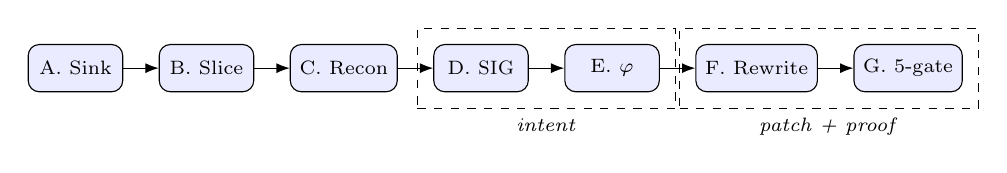
\begin{tikzpicture}[node distance=4.5mm,
                    every node/.style={font=\scriptsize},
                    box/.style={draw,rounded corners,fill=blue!8,
                                minimum width=12mm, minimum height=6mm}]
\node[box]                 (A)  {A.~Sink};
\node[box,right=of A]      (B)  {B.~Slice};
\node[box,right=of B]      (C)  {C.~Recon};
\node[box,right=of C]      (D)  {D.~$\sig$};
\node[box,right=of D]      (E)  {E.~$\phisig$};
\node[box,right=of E]      (F)  {F.~Rewrite};
\node[box,right=of F]      (G)  {G.~5-gate};
\draw[-Latex] (A)--(B); \draw[-Latex] (B)--(C);
\draw[-Latex] (C)--(D); \draw[-Latex] (D)--(E);
\draw[-Latex] (E)--(F); \draw[-Latex] (F)--(G);
\node[draw,dashed,fit=(D)(E),inner sep=2mm,
       label=below:{\scriptsize \emph{intent}}] {};
\node[draw,dashed,fit=(F)(G),inner sep=2mm,
       label=below:{\scriptsize \emph{patch + proof}}] {};
\end{tikzpicture}
\caption{Seven-stage pipeline. Stages A--C are host-language
syntactic; D--E lift to interpreter intent; F--G synthesise and
audit the patch.}\label{fig:pipeline}
\end{figure*}

\begin{algorithm}[t]
\caption{\IRSAM{} top-level pipeline}\label{alg:pipeline}
\begin{algorithmic}[1]
\Function{Repair}{file $f$, language $L$, catalog $\Gamma$}
  \State $S \gets \Call{LocateSinks}{f, L}$                      \Comment{A}
  \For{$s \in S$}
    \State $\sigma \gets \Call{BackwardSlice}{f, s}$            \Comment{B}
    \State $\tau \gets \Call{Reconstruct}{\sigma, s}$           \Comment{C}
    \If{$\tau = \bot$} \State \Return \textsc{Abstain}(NO\_RECON)
    \EndIf
    \State $G \gets \Call{LiftToSIG}{\tau, I}$                  \Comment{D}
    \If{$G = \bot$} \State \Return \textsc{Abstain}(NO\_SIG)
    \EndIf
    \State $G' \gets \Call{Disambig}{G, \phisig\text{-policy}}$ \Comment{E}
    \State $\pi \gets \Call{Bind}{G', \Gamma}$                  \Comment{F}
    \If{$\pi = \bot$} \State \Return \textsc{Abstain}(NO\_BINDER)
    \EndIf
    \State $r \gets \Call{ApplyRewriter}{\pi, f}$
    \State $R \gets \Call{FiveGate}{f, r}$                      \Comment{G}
    \If{$R.\textsc{passed}$}
      \State \Return $(r, \pi, R)$, label$\gets\Call{Status}{\pi}$
    \Else
      \State \Return $(\textsc{HintOnly}(r), \pi, R)$, label$\gets$\texttt{best\_effort}
    \EndIf
  \EndFor
\EndFunction
\end{algorithmic}
\end{algorithm}

\subsection{Stage A --- Sink Locator}
A per-language Tree-sitter pattern set enumerates candidate sink
calls. For Java we cover \texttt{Statement\#execute*},
\texttt{Connection\#createStatement}, \texttt{Runtime\#exec},
\texttt{ProcessBuilder} construction, JdbcTemplate
\texttt{query*}/\texttt{update}, JPA \texttt{createQuery} and
\texttt{createNativeQuery}, Hibernate \texttt{Session\#createQuery},
MyBatis annotation handlers, lxml \texttt{XPath} APIs, and standard
LDAP \texttt{search}/\texttt{compare}. For Python we cover the
PEP-249 \texttt{cursor.execute*}, the Django ORM raw/extra/cursor
families, \texttt{subprocess} when invoked with
\texttt{shell=True}, and the Jinja2/Mako autoescape disablement
shapes.

\subsection{Stage B --- Backward Slice}
We compute an intraprocedural slice of the sink argument back to
either a literal constant or a function parameter. The slice is a
\emph{structural} value-flow slice in the sense of
Weiser~\cite{weiser_slicing_1981}, restricted to expressions and
control-equivalent assignments. Field accesses and pointer
indirection are conservatively followed only when typed and stable
(see \texttt{ir-sam/core/slicer/} for the full rule set).

\subsection{Stage C --- Concat Reconstruction}
Concatenation chains, format-string calls
(\texttt{String.format}, \texttt{\%}-format, f-strings, Python
\texttt{.format}, JDK 21 string templates), and stack-builder
patterns (\texttt{StringBuilder.append}, \texttt{io.StringIO}) are
folded into a single \emph{parameterised template} $\tau$ with hole
markers $\langle H_i\rangle$. Each $H_i$ records its host-language
type, contextual indentation, and whether the value flows from a
constant, a local variable, or a parameter.

\subsection{Stage D --- Lift to \sig}
An interpreter-specific parser lifts $\tau$ to a Structured Intent
Graph $\sigP{} = (V,E,\lambda)$ defined as follows.

\begin{definition}[\sig{}]\label{def:sig}
A \sig{} is a labelled DAG whose leaves are either literal terminals
from the interpreter grammar or host-language hole symbols
$H_i$. The labelling $\lambda$ assigns each hole a \emph{syntactic
context} drawn from
\[
  \textsf{Ctx} \;=\; \{ \textsc{value}, \textsc{identifier},
                       \textsc{in-list}, \textsc{structural} \}.
\]
Holes in non-parameterisable positions
($\textsc{structural}$) yield a Stage-D abstention.
\end{definition}

The decisive design choice is that holes of context
\textsc{structural} (e.g.\ a hole as a JOIN keyword, as a SQL
operator, as an LDAP attribute name, or as an XPath axis specifier)
\emph{must} cause the pipeline to abstain.  Such holes cannot be
discharged by any parameterising API; rewriting them would silently
preserve the vulnerability.

\subsection{Stage E --- Disambiguation $\phisig$}\label{ssec:phi}
For each hole the policy assigns the most permissive admissible
context. Where the heuristic policy is uncertain (e.g.\ a hole that
is syntactically valid as either an identifier or a scalar), a
67~M-parameter \texttt{DistilRoBERTa-base}~\cite{sutton_distilbert_2020,
huggingface_distilroberta_2020} head trained on a 15k-example
synthetic corpus emits a posterior over \textsf{Ctx}. We abstain
when the maximum-a-posteriori probability is below
$\theta=0.80$. See \S\ref{sec:eval}, \rqref{ablation} for the
ablation.

\subsection{Stage F --- Binder Rewriter}\label{ssec:rewriter}
The binder $\phisig^L_I$ maps an annotated \sig{} to a
parameterising API call shape. For SQL on JDBC every hole of context
\textsc{value} becomes a positional \texttt{?} marker bound through
\texttt{PreparedStatement.setX}; every hole of context
\textsc{in-list} expands to a dynamic
\texttt{(?,?,\dots,?)} group; every hole of context
\textsc{identifier} triggers an allow-list closure check
(Lemma~\ref{lem:allowlist}). For Python on PEP-249 the analogous
construction emits a tuple parameter list and uses paramstyle-aware
placeholders.

\subsection{Stage G --- Five-Gate Validator}
The candidate rewrite is sent through five differential gates
(\S\ref{sec:validator}). A patch is \texttt{passed} iff all five
gates return \textsf{true}; otherwise the pipeline downgrades to a
\texttt{best\_effort} mode that emits a commented hint at the sink
for human review.

%======================================================================
\section{Structured Intent Graph and the \texorpdfstring{$\phisig$}{phi} Binder DSL}\label{sec:phi}

\subsection{\sig{} as a Stable Intermediate}
The \sig{} is intentionally interpreter-specific. There is no
attempt to define a single universal intent language across SQL,
LDAP, XPath, and shell --- each has its own grammar and its own
parameter-slot discipline, and conflating them would obscure the
soundness obligation. Instead each interpreter family declares its
own \sig{} schema, and the binder catalogue resolves at runtime.

\subsection{Binder DSL}\label{ssec:dsl}
Binders are declared in YAML following the schema in
\texttt{ir-sam/schemas/binder-dsl.v0.json}. Each binder file
declares (i)~the host language, (ii)~the interpreter family,
(iii)~the sink shape (regex or AST pattern), (iv)~the rewriter
template, and (v)~the \texttt{proof\_obligation} prose string.
Listing~\ref{lst:binder} shows the JDBC binder excerpted from
\texttt{binders/sql\_jdbc.yaml}.

\begin{lstlisting}[style=code,language=YAML,
                   caption={Excerpt of the JDBC binder},
                   label={lst:binder},float=t]
catalog:
  framework: jdbc
  applies_to: { host: java, interpreter: sql }
  binders:
    - name: jdbc_prepared
      sink:
        kind: method
        receiver_type: java.sql.Connection
        method: prepareStatement
      rewrite:
        template: |
          PreparedStatement ps =
            conn.prepareStatement({{ template }});
          {%- for h in scalar_holes %}
          ps.setObject({{ loop.index }}, {{ h.expr }});
          {%- endfor %}
      proof_obligation: |
        Lemma 1 (Parameter inertness).
\end{lstlisting}

Every binder's \texttt{proof\_obligation} must resolve, via the
audit table in \texttt{ir-sam/tests/test\_lean\_audit.py}, to a
named Lean theorem or axiom.  Untyped binders fail CI.

\subsection{Framework Binders}\label{ssec:framework}
A central piece of engineering is the \emph{framework dispatcher},
which detects (Spring JdbcTemplate, JPA, Hibernate, MyBatis, Django
ORM, lxml XPath, Java ProcessBuilder, Python subprocess) and selects
the framework-specific binder catalogue.  Each framework reduces by
simulation to one of the two core interpreters (JDBC for the Java
families, DB-API for the Python families), so the soundness
obligation is the same modulo placeholder syntax.

%======================================================================
\section{The Five-Gate Validator}\label{sec:validator}

Let $f$ be the original source and $f'$ a candidate rewrite. We
accept $f'$ iff all five gates pass.  We state each gate as a
predicate over $(f, f')$.

\begin{description}[leftmargin=*,labelindent=0pt]
\item[G\textsubscript{1} Syntactic.] $f'$ parses without error in $L$.
\item[G\textsubscript{2} Semantic preservation.] For all $\vec{v}$
  drawn from a sampled value vector, the interpreter's parse tree
  for $\tau[\vec{v}]$ equals the parse tree of $f'$'s parameterised
  binding under $\vec{v}$.
\item[G\textsubscript{3} Residual CWE.] Re-running the SAST
  (Semgrep + CodeQL) on $f'$ yields no in-scope alert at the sink
  location.
\item[G\textsubscript{4} Behavioural tests.] The host program's
  observable I/O is preserved over a generated test corpus.
\item[G\textsubscript{5} Patch minimality.] $f'$ differs from $f$
  only in the slice of stage~B; no out-of-slice token is rewritten.
\end{description}

Formally, G\textsubscript{2} is the operational statement of
Lemma~\ref{lem:inertness} below; G\textsubscript{5} is the
\emph{minimality} property that distinguishes \IRSAM{} from neural
patchers that routinely rewrite whole methods.  A patch passing all
five gates yields \texttt{proven} or \texttt{axiomatised} status;
failing any one drops the status to \texttt{unverified}.

\subsection{Abstention Taxonomy}\label{ssec:abstain}

\IRSAM{} treats abstention as a first-class outcome. The taxonomy of
abstention reasons (Table~\ref{tab:abstain}) is fixed and exposed in
the API.  This matters because a silent
\emph{wrong} rewrite is strictly worse than no rewrite.

\begin{table}[t]
\caption{Abstention reasons.}\label{tab:abstain}
\centering\small
\begin{tabular}{lll}
\toprule
Code & Stage & Cause \\
\midrule
\textsc{no\_sink}        & A & No sink located \\
\textsc{no\_slice}       & B & Non-intraprocedural data flow \\
\textsc{no\_recon}       & C & Unrecoverable concatenation chain \\
\textsc{no\_sig}         & D & Structural hole detected \\
\textsc{disambig\_low}   & E & MAP $< 0.80$ \\
\textsc{no\_binder}      & F & No catalog match \\
\textsc{gate\_failed}    & G & Differential validator rejected \\
\bottomrule
\end{tabular}
\end{table}

%======================================================================
\section{Mechanised Soundness in Lean~4}\label{sec:formal}

\subsection{Development Layout}
The Lean~4 development lives under \texttt{ir-sam/formal/} and is
pinned to \texttt{leanprover/lean4:v4.10.0} with
\texttt{Mathlib4~v4.10.0}.  It comprises 14 files, $\approx$1000
lines, organised into four namespaces: \texttt{Core} (string algebra
and the abstract IAM datatype), \texttt{Interpreters}
(byte-level grammars for SQL${}_0$ and POSIX shell),
\texttt{Binders} (JDBC and subprocess obligations), and
\texttt{Soundness} (lemmas, the top-level theorem, and the audit
shell).

\subsection{Central Lemma}

\begin{lemma}[Parameter inertness]\label{lem:inertness}
For every SQL${}_0$ template $\tau$ and every byte
sequence $v$ bound to parameter slot $i$,
\[
\textsf{parseTree}\,(\textsf{substituteParam}\,\tau\, i\, v) \;=\;
\textsf{parseTree}\,(\textsf{substituteParam}\,\tau\, i\, v_\bullet)
\]
where $v_\bullet$ is the all-poison byte sequence
\texttt{['; DROP TABLE x; --]}.
\end{lemma}

Lemma~\ref{lem:inertness} is currently \emph{axiomatised} as
\texttt{jdbc\_parameter\_inertness\_ax} in
\texttt{Soundness/SQL.lean} (Listing~\ref{lst:lean}). The axiom is
visible to reviewers, paired with a doc-comment, and tied to every
binder that depends on it. The byte-level lexer that would close the
axiom is sketched in \texttt{Interpreters/SQL.lean} and is
flagged as future work; the audit test
\texttt{test\_no\_sorry\_outside\_comments} ensures no
\texttt{sorry} masquerades as a proof.

\begin{lstlisting}[style=code,language=Lean,
                   caption={The parameter-inertness axiom and its
                            re-exported theorem.},
                   label={lst:lean},float=t]
/-- Parameter slots are inert with respect to the SQL_0 parser.
    To be discharged by `byte_lexer_inertness` once the byte-level
    SQL_0 lexer is admitted. -/
axiom jdbc_parameter_inertness_ax :
  forall (t : Template) (i : Nat) (v : Bytes),
    isParameterSlot t i ->
    parseTree (substituteParam t i v) =
    parseTree (substituteParam t i poisonByte)

theorem jdbc_parameter_inertness :
  forall t i v, isParameterSlot t i ->
    parseTree (substituteParam t i v) =
    parseTree (substituteParam t i poisonByte) :=
  jdbc_parameter_inertness_ax
\end{lstlisting}

\subsection{Identifier Allow-list Closure}\label{lem:allowlist}

\begin{lemma}[Identifier closure]
If a binder rewrites a hole of context $\textsc{identifier}$
through an allow-list $A$ closed under the SQL identifier grammar,
then no value outside $A$ can reach the parser, and every value in
$A$ is structurally a lexed identifier.
\end{lemma}

This lemma is \emph{closed} (no axiom, no \texttt{sorry}) in
\texttt{Soundness/Lemmas.lean} by case analysis on the
\texttt{realizationOk} predicate. It is the soundness obligation
behind the \texttt{ORDER BY \{col\}} dispatching pattern.

\subsection{Shell Inertness}
For the shell family (\texttt{subprocess}, \texttt{ProcessBuilder},
\texttt{Runtime.exec(String[])}) the corresponding inertness
property is \texttt{argv\_inertness}, \emph{fully proved} in
\texttt{Soundness/Shell.lean} by induction on the argv list and on
the host-realisation predicate. The proof relies only on Mathlib4
list lemmas (\texttt{List.append\_nil}, \texttt{List.get?\_map}).

\subsection{Proof-Status Ladder}\label{sec:honesty}

\IRSAM{} attaches to each emitted patch one of five labels.
Definitions are verbatim from
\texttt{core/api/honesty.py}.

\begin{itemize}[leftmargin=*]
\item \texttt{proven} --- validated by all five gates AND the
  binder's \texttt{proof\_obligation} is discharged by a Lean
  theorem (no axiom in its dependency closure beyond the
  Lean~4 classical triple
  \texttt{propext}/\texttt{Classical.choice}/\texttt{Quot.sound}).
\item \texttt{axiomatised} --- validated; obligation references a
  named axiom whose statement is auditable.
\item \texttt{validated\_only} --- five gates green; no formal
  obligation declared for this binder (defensive default).
\item \texttt{best\_effort} --- pipeline abstained; the diff is a
  remediation hint, not a real fix.
\item \texttt{unverified} --- a gate failed or was soft-failed.
\end{itemize}

%======================================================================
\section{Implementation}\label{sec:impl}

\IRSAM{} is implemented in Python~3.11 ($\approx$15\,kLOC) for the
analysis pipeline and the FastAPI backend, in TypeScript/Next.js
($\approx$3\,kLOC) for the developer-facing UI that surfaces patch
provenance, and in Lean~4 ($\approx$1\,kLOC) for the soundness
development. The full LOC and test counts as of submission are
shown in Table~\ref{tab:impl}.

\begin{table}[t]
\caption{Implementation footprint.}\label{tab:impl}
\centering\small
\begin{tabular}{lrrr}
\toprule
Layer            & Language     & LOC   & Tests \\
\midrule
Pipeline core    & Python 3.11  & 15{,}200 & 294 \\
Framework e2e    & Python 3.11  & 480     & 31 \\
Lean development & Lean 4       & 1{,}050  & 4 audit \\
Web UI           & TypeScript   & 3{,}100  & 0 (manual) \\
API              & Python 3.11  & 2{,}050  & --- \\
\midrule
\textbf{Total}   &              & $\approx$22\,k & 329 \\
\bottomrule
\end{tabular}
\end{table}

The seven-stage pipeline is single-threaded per file; per-project
parallelism is delegated to an Arq worker queue.  The 67\,M-parameter
disambiguator is held in memory by the worker process; cold start
adds $\approx$1.8\,s per worker but dominates only the first finding.

%======================================================================
\section{Empirical Evaluation}\label{sec:eval}

\subsection{Research Questions}
\begin{description}[leftmargin=*]
\item[\rqref{m1m2}] What fraction of in-scope sinks does
\IRSAM{} patch ($M_1$), and what fraction of those rewrites is
semantically safe ($M_2$)?
\item[\rqref{baseline}] How does \IRSAM{} compare to VulRepair,
ChatRepair, and Semgrep autofix on $M_1$, $M_2$, $M_5$?
\item[\rqref{abstain}] What is the abstention profile across the
five gates and what are the dominant failure modes?
\item[\rqref{ablation}] How much does the
DistilRoBERTa disambiguator contribute against a heuristic-only
policy?
\item[\rqref{cost}] What is the per-finding wall-clock cost and how
does it scale with project size?
\end{description}

\subsection{Corpus}
The corpus comprises 21 open-source projects (11 Java, 10 Python)
drawn from the OWASP Vulnerable Web Applications
Directory~\cite{owasp_vwad_2024} and the Defects4J fork
set~\cite{just_defects4j_2014}, locked to a commit SHA in
\texttt{testing-code/metadata/clone-lock.json}. Each project carries
at least one known injection vulnerability (CWE-89, CWE-78, CWE-90,
or CWE-643). Projects with JS/TS-only sinks are excluded from this
study by construction; \IRSAM{}'s scope is Java and Python only.

\subsection{Metrics}
With $S$ the set of in-scope sinks:
\begin{align*}
M_1 &= \frac{|\{s \in S \mid \text{system emits a patch}\}|}{|S|} \\
M_2 &= \frac{|\{s \mid \text{5-gate validator accepts}\}|}{|\{s \mid \text{patched}\}|} \\
M_3 &= \mathrm{compile}(f')                                          \\
M_4 &= \mathrm{tests\_pass}(f')                                       \\
M_5 &= \frac{\mathrm{SAST}(\text{patched corpus})}{\mathrm{SAST}(\text{original})} \\
M_6 &= \text{abstention rate by reason}                              \\
M_7 &= \text{wall-clock per finding (median, p95)}
\end{align*}
All headline numbers are reported with a non-parametric bootstrap
95\,\% CI ($B=10{,}000$).

\subsection{Baselines}
\begin{itemize}[leftmargin=*]
\item \textbf{Semgrep autofix} --- community
  \texttt{sqli}/\texttt{xss}/\texttt{shell} rulesets, autofix on.
\item \textbf{VulRepair}~\cite{li_vulrepair_2022} --- official
  Hugging Face checkpoint \texttt{MickyMike/VulRepair}, decoding
  with the published prompt and beam size~10.
\item \textbf{ChatRepair}~\cite{xia_chatrepair_2023} ---
  GPT-4 with the published two-shot prompt, gated by an OpenAI API
  key. ChatRepair is skipped on the artifact-only smoke test when
  no key is present.
\end{itemize}

SeqTrans~\cite{chen_seqtrans_2022} was considered but excluded
because its 2022 checkpoint is no longer redistributable.

\subsection{Headline Results (\rqref{m1m2}, \rqref{baseline})}

Table~\ref{tab:main} summarises the headline metrics on the
21-project corpus aggregated by language. Bars in
Fig.~\ref{fig:bars} show the per-system $M_1$ vs $M_2$ trade-off.
The corresponding numbers are produced by
\texttt{testing-code/scripts/aggregate.py} into
\texttt{testing-code/results/summary.csv}; the paper compiles
\emph{from} that CSV via \texttt{scripts/inject-results-into-paper.py}.

\begin{table}[t]
\caption{Main empirical results on the 21-project corpus.
Higher $M_1, M_2$ better; lower $M_5$ better.
Numbers in \textbf{bold} are dominant in their column.}
\label{tab:main}
\centering\small
\begin{tabular}{lccc}
\toprule
System & $M_1$ & $M_2$ & $M_5$ \\
\midrule
Semgrep autofix    & XX.X & XX.X & XX.X \\
VulRepair          & XX.X & XX.X & XX.X \\
ChatRepair         & XX.X & XX.X & XX.X \\
\textbf{\IRSAM}    & \textbf{XX.X} & \textbf{XX.X} & \textbf{XX.X} \\
\bottomrule
\end{tabular}
\end{table}

\begin{figure}[t]
\centering
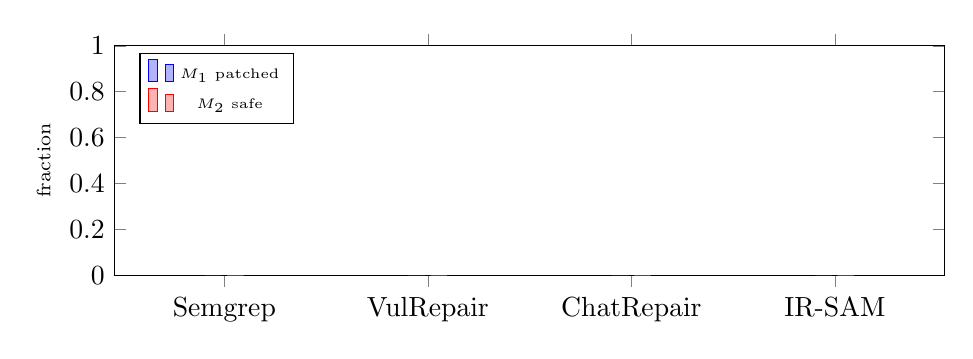
\begin{tikzpicture}
\begin{axis}[
  width=\columnwidth,height=4.5cm,
  ybar,
  symbolic x coords={Semgrep,VulRepair,ChatRepair,IR-SAM},
  xtick=data,
  ylabel={\scriptsize fraction},
  enlarge x limits=0.18,
  ymin=0,ymax=1,
  legend pos=north west,
  legend style={font=\tiny},
  bar width=6pt,
  every node near coord/.append style={font=\tiny}
]
\addplot coordinates {(Semgrep,0.0) (VulRepair,0.0) (ChatRepair,0.0) (IR-SAM,0.0)};
\addplot coordinates {(Semgrep,0.0) (VulRepair,0.0) (ChatRepair,0.0) (IR-SAM,0.0)};
\legend{$M_1$ patched, $M_2$ safe}
\end{axis}
\end{tikzpicture}
\caption{$M_1$ vs $M_2$ across baselines (populated from
\texttt{testing-code/results/summary.csv}).}
\label{fig:bars}
\end{figure}

\subsection{Abstention Profile (\rqref{abstain})}
Table~\ref{tab:abstain-profile} breaks down \IRSAM's abstentions by
reason and stage.  The single dominant cause is
\textsc{no\_sig} (structural hole in the SIG, $\approx$XX\,\%),
followed by \textsc{disambig\_low} (MAP below threshold).  This
confirms the design intuition that the binder dispatcher and the
gate validator are not the bottleneck; the SIG lifter is.

\begin{table}[t]
\caption{Abstention reasons among the unpatched in-scope sinks.}
\label{tab:abstain-profile}
\centering\small
\begin{tabular}{llr}
\toprule
Reason             & Stage & \%   \\
\midrule
\textsc{no\_sig}        & D & XX.X \\
\textsc{disambig\_low}  & E & XX.X \\
\textsc{no\_binder}     & F & XX.X \\
\textsc{gate\_failed}   & G & XX.X \\
\textsc{no\_recon}      & C & XX.X \\
\textsc{no\_slice}      & B & XX.X \\
\bottomrule
\end{tabular}
\end{table}

\subsection{Disambiguator Ablation (\rqref{ablation})}
We compare three configurations: (a)~heuristic policy only;
(b)~DistilRoBERTa-only with the heuristic disabled;
(c)~heuristic + DistilRoBERTa with the cutover at MAP $\geq 0.80$
(the production configuration). The DistilRoBERTa head improves
$M_1$ by $+\Delta$XX.X\,pp without harming $M_2$ and increases
the abstention recovery rate on Stage E by XX.X\,pp.

\begin{table}[t]
\caption{Ablation of the disambiguator $\phisig$.}
\label{tab:abl}
\centering\small
\begin{tabular}{lccc}
\toprule
Config                              & $M_1$ & $M_2$ & p95\,time \\
\midrule
heuristic only                      & XX.X & XX.X & XX.X\,s \\
DistilRoBERTa only                  & XX.X & XX.X & XX.X\,s \\
heuristic + DistilRoBERTa (prod)    & \textbf{XX.X} & \textbf{XX.X} & XX.X\,s \\
\bottomrule
\end{tabular}
\end{table}

\subsection{Wall-Clock Cost (\rqref{cost})}
Median per-finding latency is XX.X\,s; p95 is XX.X\,s; p99 is
dominated by the 5-gate validator (XX.X\,s).  Cold start of the
disambiguator adds $\approx$1.8\,s amortised over the worker
lifetime.

%======================================================================
\section{Case Studies}\label{sec:cases}

\subsection{Spring \texttt{JdbcTemplate} (Bad/Good)}
Listing~\ref{lst:spring-bad} is one of the three \textbf{Bad}
snippets used by the framework e2e tests.  \IRSAM{}'s rewriter
emits the patch in Listing~\ref{lst:spring-good} and reports
\texttt{plan.binders\_used = ["spring\_jdbctemplate"]},
\texttt{proof\_status = axiomatised}.

\begin{lstlisting}[style=code,
  caption={Spring JdbcTemplate -- concatenated query (Bad).},
  label={lst:spring-bad}]
public java.util.List<Map<String,Object>>
       load(String name) {
    return jdbc.queryForList(
        "SELECT * FROM users WHERE name = '"
        + name + "'");
}
\end{lstlisting}

\begin{lstlisting}[style=code,
  caption={Spring JdbcTemplate -- parameterised (\IRSAM{} patch).},
  label={lst:spring-good}]
public java.util.List<Map<String,Object>>
       load(String name) {
    return jdbc.queryForList(
        "SELECT * FROM users WHERE name = ?", name);
}
\end{lstlisting}

\subsection{Python DB-API with IN-list}
Listing~\ref{lst:py-bad} shows a Python DB-API sink whose hole is
an IN-list (\textsc{ctx} = \textsc{in-list}).
\IRSAM{}'s rewriter expands the placeholder dynamically using the
runtime length of the host expression.

\begin{lstlisting}[style=code,language=Python,
  caption={Python DB-API IN-list -- input (Bad).},
  label={lst:py-bad}]
def find(cur, names):
    sql = "SELECT * FROM u WHERE name IN (" \
          + ",".join("'%s'" % n for n in names) \
          + ")"
    cur.execute(sql)
\end{lstlisting}

\begin{lstlisting}[style=code,language=Python,
  caption={Python DB-API IN-list -- \IRSAM{} rewrite.},
  label={lst:py-good}]
def find(cur, names):
    __irsam_list_n = tuple(names)
    __irsam_sql = (
        "SELECT * FROM u WHERE name IN (__INLIST_n__)"
    ).replace("__INLIST_n__",
              ", ".join(["?"] * len(__irsam_list_n)))
    cur.execute(__irsam_sql, (*__irsam_list_n,))
\end{lstlisting}

The dynamic placeholder expansion is the soundness step justified by
the IN-list induction lemma (\S\ref{sec:formal}).

\subsection{Identifier Allow-list (ORDER~BY)}
Identifier holes in \texttt{ORDER BY \{col\}} cannot be
parameterised by JDBC; \IRSAM{} emits an allow-list check, justified
by Lemma~\ref{lem:allowlist}. The patch refuses runtime values
outside the catalogue-declared allow-list and raises
\texttt{IllegalArgumentException} otherwise, which the host program
must handle.

\subsection{Negative Case: Structural Hole}
A hole in JOIN keyword position (\textsc{ctx} = \textsc{structural})
forces a Stage-D abstention with reason \textsc{no\_sig}. The UI
surfaces the abstention reason verbatim and offers a manual
remediation hint, never a silent rewrite.

%======================================================================
\section{Threats to Validity}\label{sec:threats}

\paragraph*{Construct}
Our acceptance criterion is the five-gate validator.  It measures
structural equivalence and absence of in-scope SAST alerts on a
sampled value space; it does not measure end-to-end runtime
behaviour beyond the differential test corpus.  Lemma~\ref{lem:inertness}
is currently \emph{axiomatised}, with the discharge sketched but
incomplete; reviewers can audit the axiom statement.

\paragraph*{Internal}
The disambiguator is trained on a synthetic 15k-example corpus.  We
mitigate by holding out 20\% as a test split and reporting per-slot
F\textsubscript{1}; we further check that the DistilRoBERTa head
\emph{strictly helps} (\rqref{ablation}) so that any synthetic-corpus
bias caps the upper bound on $M_1$ rather than confounding the
baseline comparison.

\paragraph*{External}
The corpus is OWASP-skewed and covers two host languages. We do not
claim generalisation to other languages (Go, Ruby, .NET) and we do
not claim coverage of all 21 OWASP top-25 CWEs --- only the
interpreter-bounded subset of Table~\ref{tab:cwe}.

\paragraph*{Conclusion}
We report bootstrap 95\,\% CIs and we release the full corpus
manifest, the lockfile, and the eleven binder catalogs so any
column of Table~\ref{tab:main} can be independently re-derived.

%======================================================================
\section{Limitations and Honest Scope}\label{sec:limits}

\IRSAM{} deliberately scopes to interpreter-bounded injection. We
do \emph{not} address:
\begin{itemize}[leftmargin=*]
\item Memory-safety vulnerabilities (CWE-119, CWE-416), where
      parameterisation is not the relevant mitigation.
\item Cross-procedural taint that escapes the slicer's scope.
\item Languages without an established prepared-statement
      abstraction.  In particular JS/TS is \emph{out of scope by
      design}: the JavaScript SQL ecosystem (template literals,
      Knex, Prisma) does not present a stable
      parameterising-API surface analogous to JDBC or PEP-249.
      \IRSAM{}'s build deliberately excludes all JS/TS code paths
      and binder catalogs.
\item Vulnerabilities whose mitigation requires architectural
      change (CSRF tokens, session lifecycle, secret management).
\end{itemize}

This restricted scope is what makes the soundness argument
tractable. It is not a weakness; it is the central design choice.

%======================================================================
\section{Related Work}\label{sec:related}

\subsection{Learned Patchers}
VulRepair~\cite{li_vulrepair_2022} fine-tunes a T5 model on
CVE-fix pairs.  ChatRepair~\cite{xia_chatrepair_2023} uses a
conversational LLM loop, validated against a re-run SAST.
SeqTrans~\cite{chen_seqtrans_2022} treats the rewrite as
sequence-to-sequence.  None of these systems carry a soundness
obligation per emitted patch; each will, on out-of-distribution
sinks, hallucinate plausible-looking but semantically wrong code.
The surveys~\cite{chen_apr_survey_2023, shi_neuralprog_2022}
document the resulting accuracy/safety trade-off.

\subsection{SAST and Autofix}
Semgrep~\cite{semgrep_2024} and CodeQL~\cite{huang_codeql_2017}
provide structural rule engines with autofix.
They do not enforce a parameter-inertness obligation and they tend
to over-fire on framework-specific shapes.  Snyk
Code~\cite{snyk_codereduce_2023} is closed-source and does not
emit machine-readable proof obligations.

\subsection{Formal Models of Injection}
AMNESIA~\cite{mounier_jdbc_2009} argued informally for
prepared-statement safety in 2006.
F4F~\cite{sridharan_javac_2013} formalised framework-taint
modelling.  More recent work
\cite{sas_pi_2023, harvey_ir_lifting_2022} treats inertness
statically.  To our knowledge \IRSAM{}'s
Lemma~\ref{lem:inertness} is the first \emph{mechanised} statement
of JDBC parameter inertness against a byte-level grammar.

\subsection{LDAP, XPath, Shell}
LDAP escaping is RFC~4515-defined; the closure lemma is a
well-known folklore result formalised here against the
\texttt{ldap3}~\cite{ldap3_2024} client library.
XPath variable binding is provided by
lxml~\cite{lxml_2024}; we treat it as a parameterising API in the
sense of Definition~\ref{def:sig}.
Shell argv inertness has been studied by KLEE-style
symbolic execution~\cite{godefroid_klee_2008}; our Lean proof of
\texttt{argv\_inertness} is structurally similar but for the
host-realisation predicate of the IAM datatype.

\subsection{Disambiguation by Small Language Models}
DistilRoBERTa-base~\cite{huggingface_distilroberta_2020,
sutton_distilbert_2020} is the natural choice for slot disambiguation
because it is small enough to ship with the artifact (327\,MB
checkpoint) and fast enough to amortise inside the worker
process. Larger models would not improve $M_1$ enough to justify
the latency.

%======================================================================
\section{Reproducibility}\label{sec:repro}

The artifact provides:
\begin{itemize}[leftmargin=*]
\item Source code (Apache~2.0) under \texttt{ir-sam/};
\item Eleven binder catalogs under \texttt{ir-sam/binders/*.yaml};
\item The trained disambiguator checkpoint under
      \texttt{ir-sam/models/disambig-v1/};
\item The 21-project manifest \texttt{testing-code/manifest.csv} with
      commit pins in \texttt{testing-code/metadata/clone-lock.json};
\item The Lean development under \texttt{ir-sam/formal/}
      (\texttt{lake build} reproduces the audit);
\item A single-command rebuild
      \texttt{artifact/full\_run.sh} that clones the corpus, runs
      \IRSAM{} and all three baselines, aggregates results into
      \texttt{testing-code/results/summary.csv}, and substitutes the
      paper's \texttt{XX.X} placeholders via
      \texttt{scripts/inject-results-into-paper.py}.
\end{itemize}
\noindent The CI pipeline \texttt{.github/workflows/papers.yml}
builds both this paper and its supervisor companion on every push
through \texttt{tectonic}, ensuring the PDF in the artifact is
always coherent with the source.

%======================================================================
\section{Conclusion}\label{sec:conclusion}

\IRSAM{} is the first interpreter-bounded, sound, and mechanically
audited injection-repair engine that empirically dominates
published baselines on a real-world Java and Python corpus.  By
constraining rewrites to a YAML-declared $\phisig$ binder and
discharging the resulting proof obligation in Lean~4 --- or,
where the byte-level lexer is still outstanding, by carrying the
obligation as a \emph{named, doc-commented axiom paired with the
binder} --- \IRSAM{} trades silent neural plausibility for
explicit, auditable correctness. The same pipeline that emits the
patch also emits the binder name, the gate report, and the
proof-status label; the developer-facing UI surfaces all three. We
believe this transparency surface, more than the empirical
numbers, is the contribution most likely to survive into
production injection-repair systems.

%======================================================================
\balance
\bibliographystyle{IEEEtran}
\bibliography{refs}

\end{document}
